\documentclass[journal,12pt,twocolumn]{IEEEtran}

\usepackage{setspace}
\usepackage{gensymb}
\singlespacing
\usepackage[cmex10]{amsmath}

\usepackage{amsthm}

\usepackage{mathrsfs}
\usepackage{txfonts}
\usepackage{stfloats}
\usepackage{bm}
\usepackage{cite}
\usepackage{cases}
\usepackage{subfig}

\usepackage{longtable}
\usepackage{multirow}
\usepackage{enumitem}
\usepackage{mathtools}
\usepackage{steinmetz}
\usepackage{tikz}
\usepackage{circuitikz}
\usepackage{verbatim}
\usepackage{tfrupee}
\usepackage[breaklinks=true]{hyperref}
\usepackage{graphicx}
\usepackage{tkz-euclide}

\usetikzlibrary{calc,math}
\usepackage{listings}
    \usepackage{color}                                            %%
    \usepackage{array}                                            %%
    \usepackage{longtable}                                        %%
    \usepackage{calc}                                             %%
    \usepackage{multirow}                                         %%
    \usepackage{hhline}                                           %%
    \usepackage{ifthen}                                           %%
    \usepackage{lscape}     
\usepackage{multicol}
\usepackage{chngcntr}

\DeclareMathOperator*{\Res}{Res}

\renewcommand\thesection{\arabic{section}}
\renewcommand\thesubsection{\thesection.\arabic{subsection}}
\renewcommand\thesubsubsection{\thesubsection.\arabic{subsubsection}}

\renewcommand\thesectiondis{\arabic{section}}
\renewcommand\thesubsectiondis{\thesectiondis.\arabic{subsection}}
\renewcommand\thesubsubsectiondis{\thesubsectiondis.\arabic{sub subsection}}


\hyphenation{optical networks semiconduc-tor}
\def\inputGnumericTable{}                                 %%

\lstset{
%language=C,
frame=single, 
breaklines=true,
columns=fullflexible
}
\date{March 2021}

\begin{document}

\newcommand{\BEQA}{\begin{eqnarray}}
\newcommand{\EEQA}{\end{eqnarray}}
\newcommand{\define}{\stackrel{\triangle}{=}}
\bibliographystyle{IEEEtran}
\raggedbottom
\setlength{\parindent}{0pt}
\providecommand{\mbf}{\mathbf}
\providecommand{\pr}[1]{\ensuremath{\Pr\left(#1\right)}}
\providecommand{\qfunc}[1]{\ensuremath{Q\left(#1\right)}}
\providecommand{\fn}[1]{\ensuremath{f\left({#1}\right)}}
\providecommand{\e}[1]{\ensuremath{E\left(#1\right)}}
\providecommand{\sbrak}[1]{\ensuremath{{}\left[#1\right]}}
\providecommand{\lsbrak}[1]{\ensuremath{{}\left[#1\right.}}
\providecommand{\rsbrak}[1]{\ensuremath{{}\left.#1\right]}}
\providecommand{\brak}[1]{\ensuremath{\left(#1\right)}}
\providecommand{\lbrak}[1]{\ensuremath{\left(#1\right.}}
\providecommand{\rbrak}[1]{\ensuremath{\left.#1\right)}}
\providecommand{\cbrak}[1]{\ensuremath{\left\{#1\right\}}}
\providecommand{\lcbrak}[1]{\ensuremath{\left\{#1\right.}}
\providecommand{\rcbrak}[1]{\ensuremath{\left.#1\right\}}}
\theoremstyle{remark}
\newtheorem{rem}{Remark}
\newcommand{\sgn}{\mathop{\mathrm{sgn}}}
\newcommand{\comb}[2]{{}^{#1}\mathrm{C}_{#2}}
\providecommand{\abs}[1]{\vert#1\vert}
\providecommand{\res}[1]{\Res\displaylimits_{#1}} 
\providecommand{\norm}[1]{\lVert#1\rVert}
%\providecommand{\norm}[1]{\lVert#1\rVert}
\providecommand{\mtx}[1]{\mathbf{#1}}
\providecommand{\mean}[1]{E\sbrak{ #1 }}
\providecommand{\fourier}{\overset{\mathcal{F}}{ \rightleftharpoons}}
%\providecommand{\hilbert}{\overset{\mathcal{H}}{ \rightleftharpoons}}
\providecommand{\system}{\overset{\mathcal{H}}{ \longleftrightarrow}}
	%\newcommand{\solution}[2]{\textbf{Solution:}{#1}}
\newcommand{\solution}{\noindent \textbf{Solution: }}
\newcommand{\cosec}{\,\text{cosec}\,}
\providecommand{\dec}[2]{\ensuremath{\overset{#1}{\underset{#2}{\gtrless}}}}
\newcommand{\myvec}[1]{\ensuremath{\begin{pmatrix}#1\end{pmatrix}}}
\newcommand{\mydet}[1]{\ensuremath{\begin{vmatrix}#1\end{vmatrix}}}
\numberwithin{equation}{subsection}
\makeatletter
\@addtoreset{figure}{problem}
\makeatother
\let\StandardTheFigure\thefigure
\let\vec\mathbf
\vspace{3cm}
\title{EE3900 Assignment - 1}
\author{Adhvik Mani Sai Murarisetty - AI20BTECH11015}
\maketitle
\newpage
\bigskip
\renewcommand{\thetable}{\theenumi}

Download latex-tikz codes from 
%
\begin{lstlisting}
https://github.com/adhvik24/EE3900/blob/main/Assignment_1/Assignment_1.tex
\end{lstlisting}
%
Download python codes from 
%
\begin{lstlisting}
https://github.com/adhvik24/EE3900/blob/main/Assignment_1/Assignment1.py
\end{lstlisting}
\section{Ramsey 1.1 qn 14}
Prove that the middle point of the line joining the points $\myvec{-5\\12}$ and $\myvec{9\\-2}$ is a point of trisection of the line
joining the points $\myvec{-8\\-5}$ and $\myvec{7\\10}$.
\section{SOLUTION}
The $\vec{C}$ that divides $\vec{A},\vec{B}$ in the ratio $k:1$ is
\begin{align}
\vec{C}=\frac{k\vec{B}+\vec{A}}{k+1}\label{0}
\end{align}
Let $\vec{C}$ is the middle point of the line joining the points $\vec{A} = \myvec{-5\\12}$ and $\vec{B} = \myvec{9\\-2}$, Then $k=1$,
\begin{align}
    \vec{C}&=\frac{\vec{B}+\vec{A}}{1+1}=\frac{\vec{B}+\vec{A}}{2}\\
    &= \frac{\myvec{9\\-2}+\myvec{-5\\12}}{2}\\
    \implies \vec{C}&= \myvec{2\\5}
\end{align}
And now we have to find the ratio in which $\vec{C}$ divides the line
joining the points $\vec{P}$ = $\myvec{-8\\-5}$ and $\vec{Q}$ = $\myvec{7\\10}$. Let the ratio is $k:1$,
Then,
\begin{align}
    \implies \vec{C}&=\frac{k\vec{Q}+\vec{P}}{k+1}\\
    \myvec{2\\5} &= \frac{{k{\myvec{7\\10}+\myvec{-8\\-5}}}}{k+1}\\
    \myvec{2\\5}&=\frac{1}{k+1} \myvec{7k-8\\10k-5}\\
    \implies k &= 2
\end{align}
As $k=2$, That implies $\vec{C}$ divides the line
joining the points $\vec{P}$ = $\myvec{-8\\-5}$ and $\vec{Q}$ = $\myvec{7\\10}$ in the ratio $2:1$.

$\therefore$ $\vec{C}$  is point of trisection of line joining $\vec{P}$ and $\vec{Q}$.

\begin{figure}[htp]
    \centering
    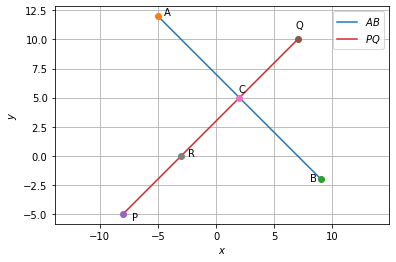
\includegraphics[width=\columnwidth]{a_1.png}
    \caption{graphical representation of points and lines} \label{a_1}
\end{figure}

$\therefore$ The middle point of the line joining the points $\myvec{-5\\12}$ and $\myvec{9\\-2}$ is a point of trisection of the line
joining the points $\myvec{-8\\-5}$ and $\myvec{7\\10}$.
\end{document}
